\documentclass[11pt,a4paper,fontset=fandol]{ctexart}

\usepackage{geometry}
\geometry{a4paper, left=2.2cm, right=2.2cm, top=2.2cm, bottom=2.2cm, headheight=14pt}
\usepackage{setspace}
\linespread{1.05}
\usepackage{indentfirst}
\setlength{\parindent}{2em}
\emergencystretch=2em
\sloppy

\usepackage{xcolor}
\definecolor{themecolor}{RGB}{40,90,140}
\definecolor{codebg}{RGB}{248,248,245}

\usepackage{graphicx}
\graphicspath{{results/}}
\usepackage{amsmath}
\usepackage{booktabs}
\usepackage{caption}
\captionsetup{font=small,labelfont={bf,color=themecolor}}
\usepackage{subcaption}
\usepackage{float}
\usepackage{array}
\usepackage{verbatim}
\usepackage{hyperref}
\hypersetup{
  colorlinks=true,
  linkcolor=themecolor,
  citecolor=themecolor,
  urlcolor=themecolor!70!black,
}

\usepackage{titlesec}
\titleformat{\section}
  {\color{themecolor}\bfseries\fontsize{13}{16}\selectfont}
  {\thesection}{0.6em}{}
\titlespacing*{\section}{0pt}{0.9em}{0.35em}

\titleformat{\subsection}
  {\color{themecolor!85!black}\bfseries\fontsize{11.5}{14}\selectfont}
  {\thesubsection}{0.6em}{}
\titlespacing*{\subsection}{0pt}{0.55em}{0.15em}

\usepackage{fancyhdr}
\pagestyle{fancy}
\fancyhf{}
\renewcommand{\headrulewidth}{0.4pt}
\lhead{\small\color{black!55} 地图构建与定位实验报告}
\rhead{\small\color{black!55} 人工智能 2302}
\cfoot{\small\color{black!55}\thepage}

\fancypagestyle{plain}{
  \fancyhf{}
  \renewcommand{\headrulewidth}{0pt}
  \cfoot{\small\color{black!55}\thepage}
}

\usepackage{mdframed}
\BeforeBeginEnvironment{verbatim}{
  \begin{mdframed}[
    backgroundcolor=codebg,
    linecolor=themecolor!30,
    linewidth=0.5pt,
    innerleftmargin=10pt,
    innerrightmargin=8pt,
    innertopmargin=6pt,
    innerbottommargin=4pt,
    skipabove=8pt,
    skipbelow=8pt,
    roundcorner=2pt,
  ]
}
\AfterEndEnvironment{verbatim}{\end{mdframed}}

\setCJKmonofont{Arial Unicode MS}

\title{\bfseries 地图构建与定位实验报告}
\author{人工智能2302 \quad 蒋梓轩\\
人工智能2302 \quad 汪翌秦\\
人工智能2302 \quad 孙靖淞}
\date{2026 年 5 月 29 日}

\begin{document}

\maketitle

\section{实验目的}

实验 3 与实验 4 是一条连续的导航前置链路：先在仿真与实车环境中利用激光雷达构建二维栅格地图，再在保存的静态地图上启动 AMCL，完成移动机器人全局重定位和连续位姿跟踪。本报告将两个实验合并整理，重点说明从 Gazebo/RViz 建图、地图保存，到 \verb|map_server|、RF2O、AMCL 定位验证的完整过程。

通过本组实验，需要掌握四个方面：第一，理解 \verb|/scan|、\verb|/tf|、\verb|/map| 与 \verb|/particlecloud| 在建图和定位中的作用；第二，理解 Gazebo、RViz 和 URDF 在仿真验证中的分工；第三，掌握 \verb|gmapping|、\verb|hector_mapping| 与 \verb|map_server| 的使用流程；第四，理解 \verb|map -> odom -> base_footprint| 这条 TF 链为什么是后续路径规划的基础。

\section{实验原理}

建图阶段的目标是把机器人运动过程中的激光雷达观测投影到统一坐标系中，形成占据栅格地图。仿真环境中，\verb|gmapping| 结合里程计和激光扫描估计机器人轨迹并生成 \verb|/map|；实车环境中，\verb|hector_mapping| 更依赖高频激光扫描匹配，在轮式里程计不稳定时仍能构建可用地图。地图保存后，\verb|map_server| 会根据 \verb|nav.yaml| 加载 \verb|nav.pgm|，重新发布静态地图。

定位阶段使用 AMCL 粒子滤波算法。每个粒子表示一个可能的机器人位姿，运动模型根据里程计传播粒子，观测模型根据激光扫描与静态地图的匹配程度更新粒子权重。粒子云从分散到收敛，表示机器人位姿估计从不确定逐步变得稳定。

\begin{table}[H]
  \centering
  \caption{实验 3-4 关键模块与作用}
  \begin{tabular}{lll}
    \toprule
    模块 & 主要输入 & 输出或作用 \\
    \midrule
    Gazebo/robot\_sim & 机器人模型、仿真世界 & 提供仿真运动和激光数据 \\
    \verb|gmapping| & \verb|/scan|、TF/里程计 & 构建仿真栅格地图 \\
    \verb|hector_mapping| & \verb|/scan|、雷达坐标关系 & 构建实车实验场地地图 \\
    \verb|map_server| & \verb|nav.yaml|、\verb|nav.pgm| & 发布静态地图 \verb|/map| \\
    RF2O & 激光扫描序列 & 发布局部里程计估计 \\
    AMCL & 静态地图、激光、里程计 & 发布 \verb|map -> odom| 定位修正 \\
    \bottomrule
  \end{tabular}
\end{table}

\section{实验步骤与结果分析}

\subsection{仿真环境加载与地图构建}

实验首先启动 Gazebo 仿真环境，加载带激光雷达的小车模型和包含墙体、圆柱、方块障碍物的室内场景。随后启动 \verb|slam_gmapping.launch|，通过键盘遥控机器人覆盖主要通行区域。图 \ref{fig:gazebo-map} 左图为 Gazebo 中的实验场景，右图为 RViz 中保存后的仿真地图结果，可以看到墙体和障碍物轮廓已经被较完整地写入栅格地图。

\begin{figure}[H]
  \centering
  \begin{subfigure}{0.49\linewidth}
    \centering
    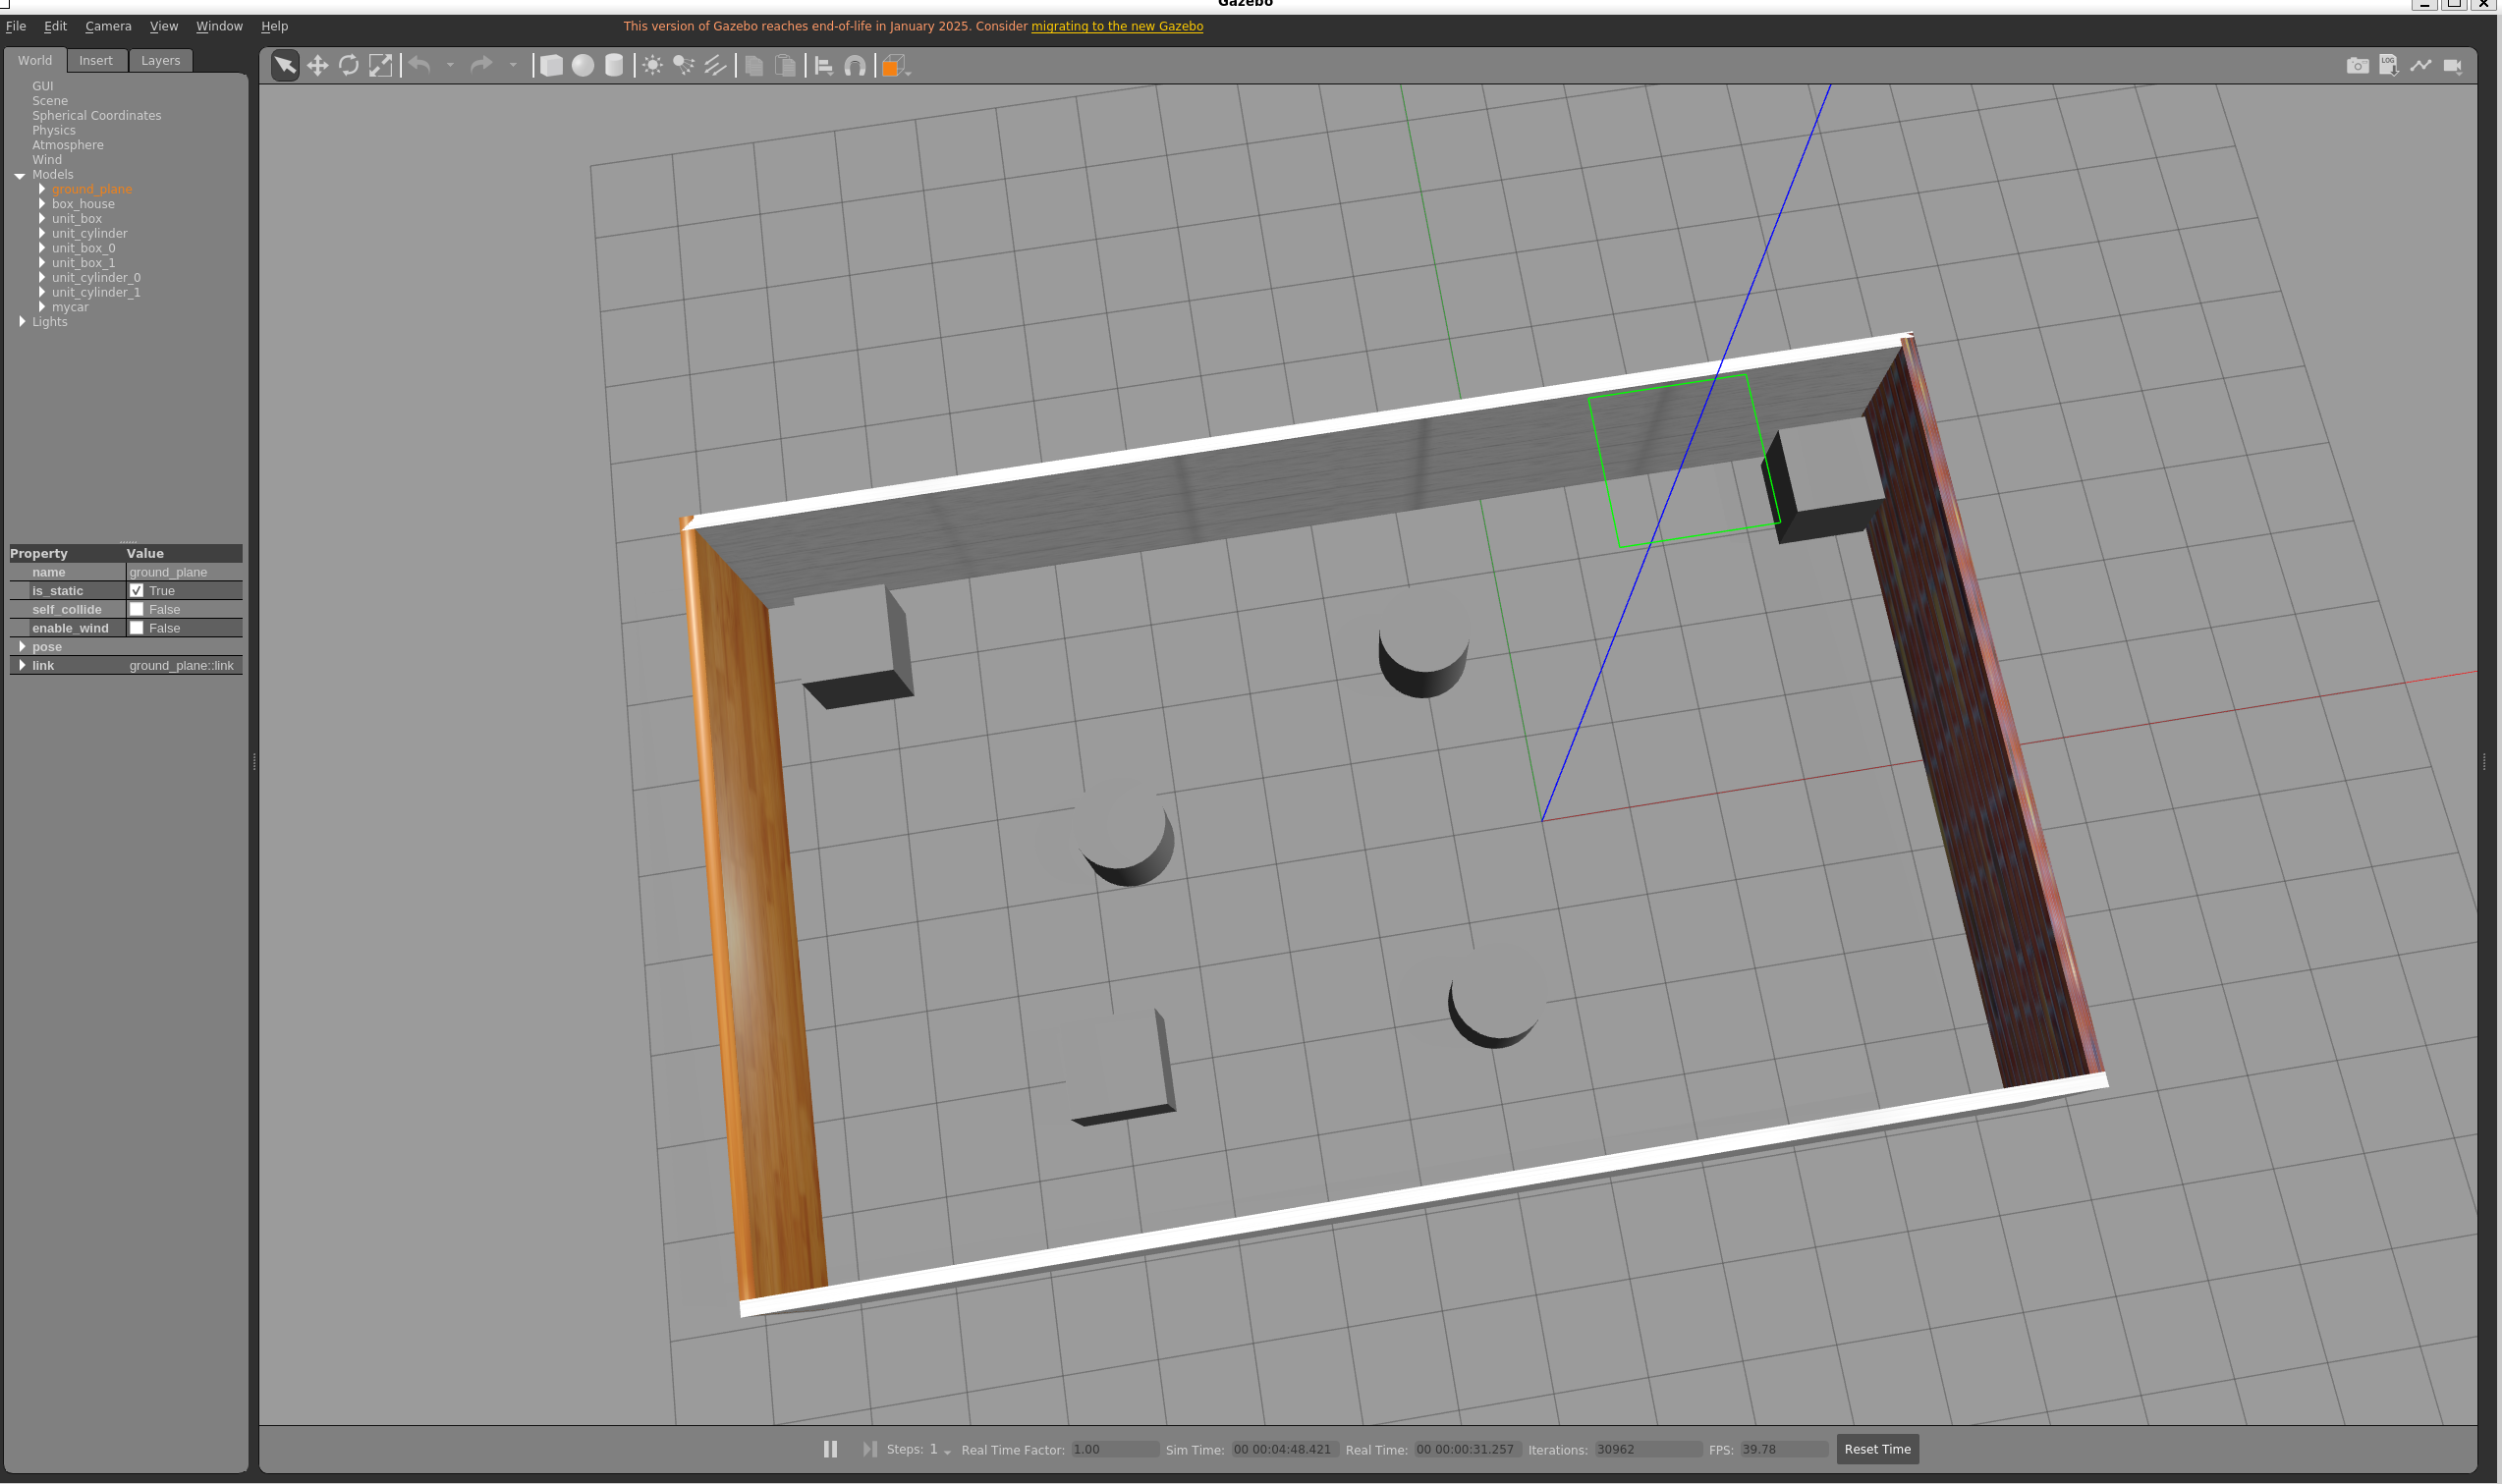
\includegraphics[width=\linewidth]{lab34_gazebo_environment.png}
    \caption{Gazebo 仿真环境}
  \end{subfigure}
  \hfill
  \begin{subfigure}{0.49\linewidth}
    \centering
    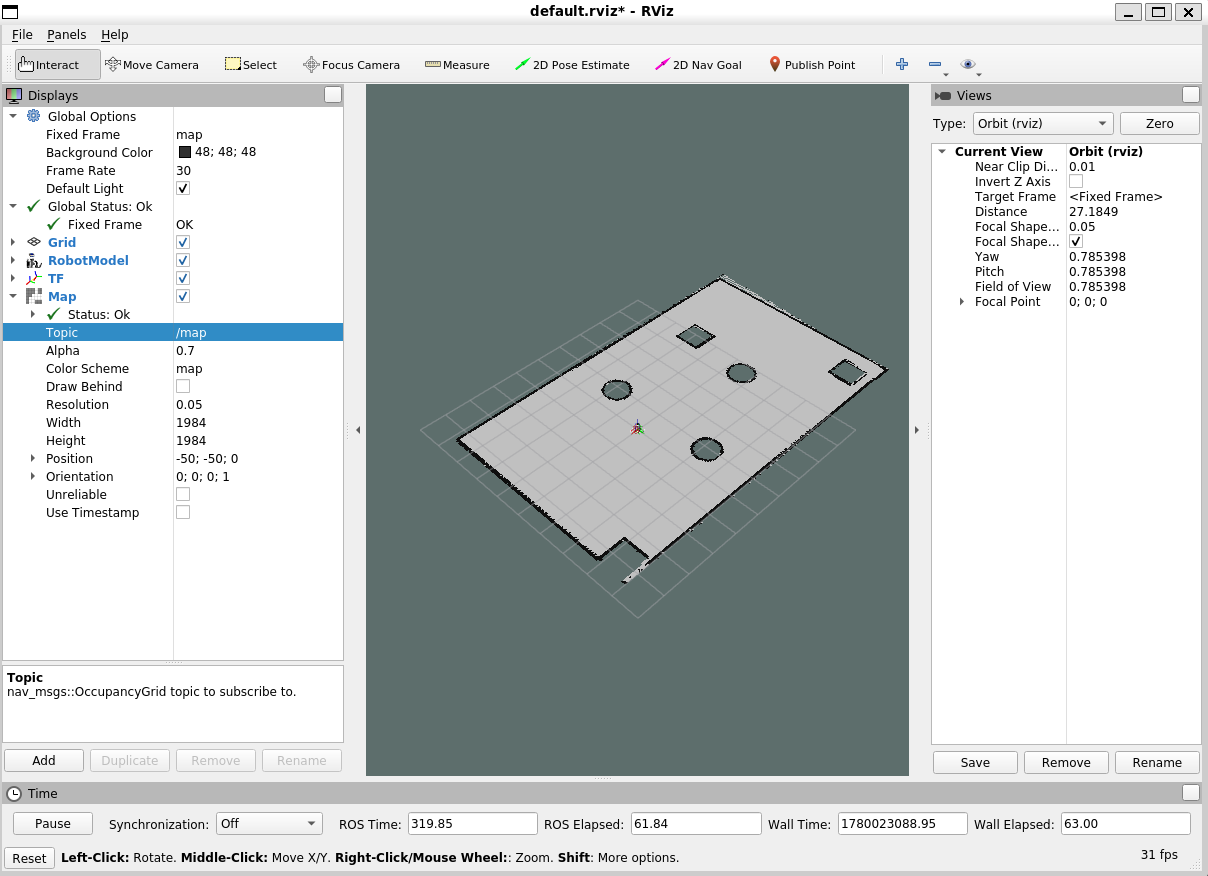
\includegraphics[width=\linewidth]{lab34_final_sim_map.png}
    \caption{RViz 中的仿真地图}
  \end{subfigure}
  \caption{实验 3 仿真环境与地图构建结果。}
  \label{fig:gazebo-map}
\end{figure}

地图构建完成后，使用 \verb|map_server| 保存地图：

\begin{verbatim}
rosrun map_server map_saver -f nav
\end{verbatim}

保存结果包括 \verb|nav.pgm| 和 \verb|nav.yaml|。其中 \verb|nav.pgm| 保存占据栅格图像，\verb|nav.yaml| 记录分辨率、原点和占据阈值。本次整理的地图分辨率为 \verb|0.05 m/cell|，后续实验 4 和实验 5 都复用该地图。

\subsection{实车建图与地图效果}

实车实验中，先通过 \verb|bringup.launch| 启动底盘、雷达和静态 TF，再启动 \verb|hector_mapping| 建图节点。相比 \verb|gmapping|，Hector 对轮式里程计依赖更小，更适合实车场景中激光扫描频率较高但轮式里程计误差较大的情况。图 \ref{fig:real-mapping} 显示了实车或远程环境下的建图过程，地图边界随机器人运动逐步扩展，局部区域存在由扫描噪声和覆盖路径不足导致的毛刺。

\begin{figure}[H]
  \centering
  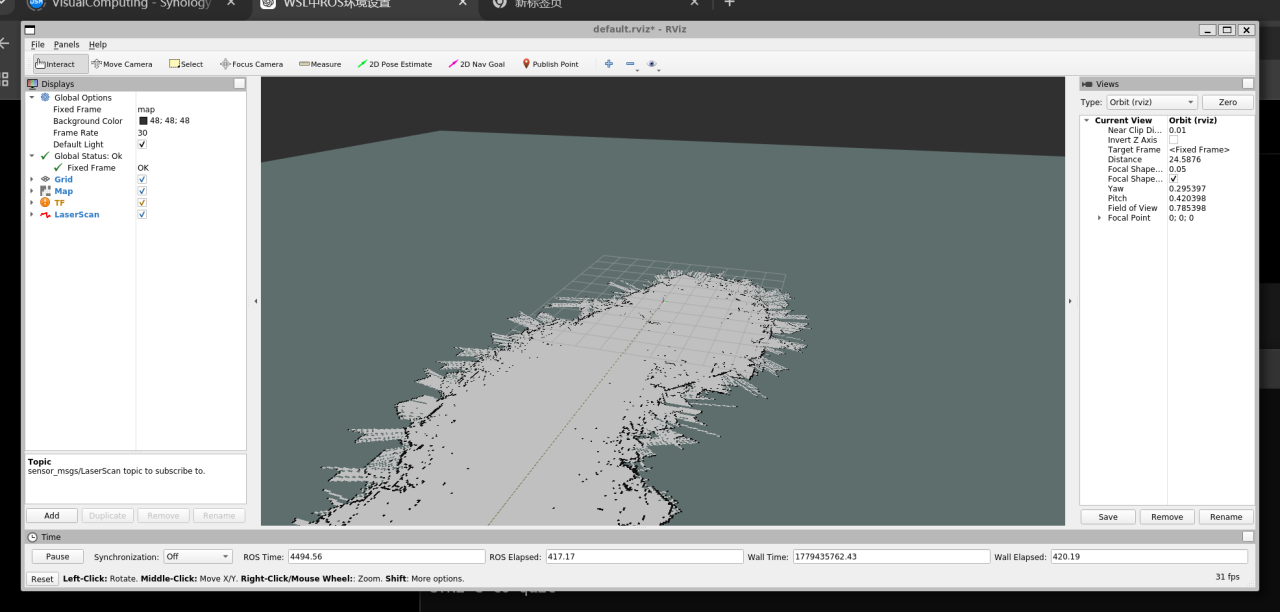
\includegraphics[width=0.88\linewidth]{lab34_hector_mapping_process.png}
  \caption{实车/远程环境中的 Hector 建图过程。}
  \label{fig:real-mapping}
\end{figure}

建图质量主要取决于三点：一是雷达与底盘之间的静态 TF 是否准确；二是机器人运动是否覆盖足够多的观察角度；三是地图分辨率和扫描匹配参数是否适中。若雷达坐标系标定错误，障碍物会被投影到错误位置，地图容易出现重影、墙体弯曲或闭合失败。

\subsection{静态地图定位与粒子云收敛}

定位实验在已保存地图上启动 \verb|test_amcl.launch|。该 launch 文件加载 \verb|map_server|、RF2O 激光里程计和 AMCL，使系统形成 \verb|map -> odom -> base_footprint| 的坐标链。RViz 中添加 Map、LaserScan、TF、RobotModel 和 PoseArray 后，可以同时观察地图、激光点、机器人模型和粒子云。

图 \ref{fig:amcl-sim} 左图显示地图、激光和 TF 已经在 \verb|map| 坐标系下对齐；中图显示初始粒子云较分散，表示位姿不确定性较高；右图显示经过运动和激光匹配后粒子云收缩到机器人附近，说明 AMCL 定位开始收敛。

\begin{figure}[H]
  \centering
  \begin{subfigure}{0.32\linewidth}
    \centering
    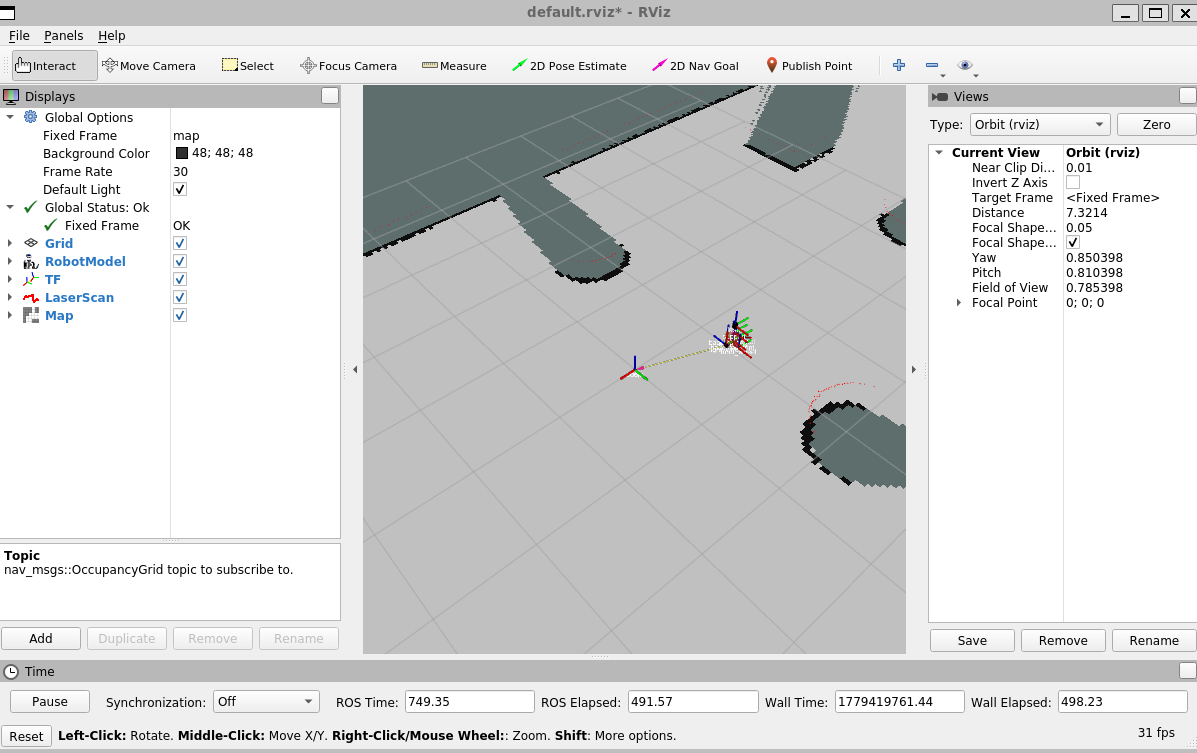
\includegraphics[width=\linewidth]{lab34_localization_scan_tf.png}
    \caption{地图、激光与 TF}
  \end{subfigure}
  \hfill
  \begin{subfigure}{0.32\linewidth}
    \centering
    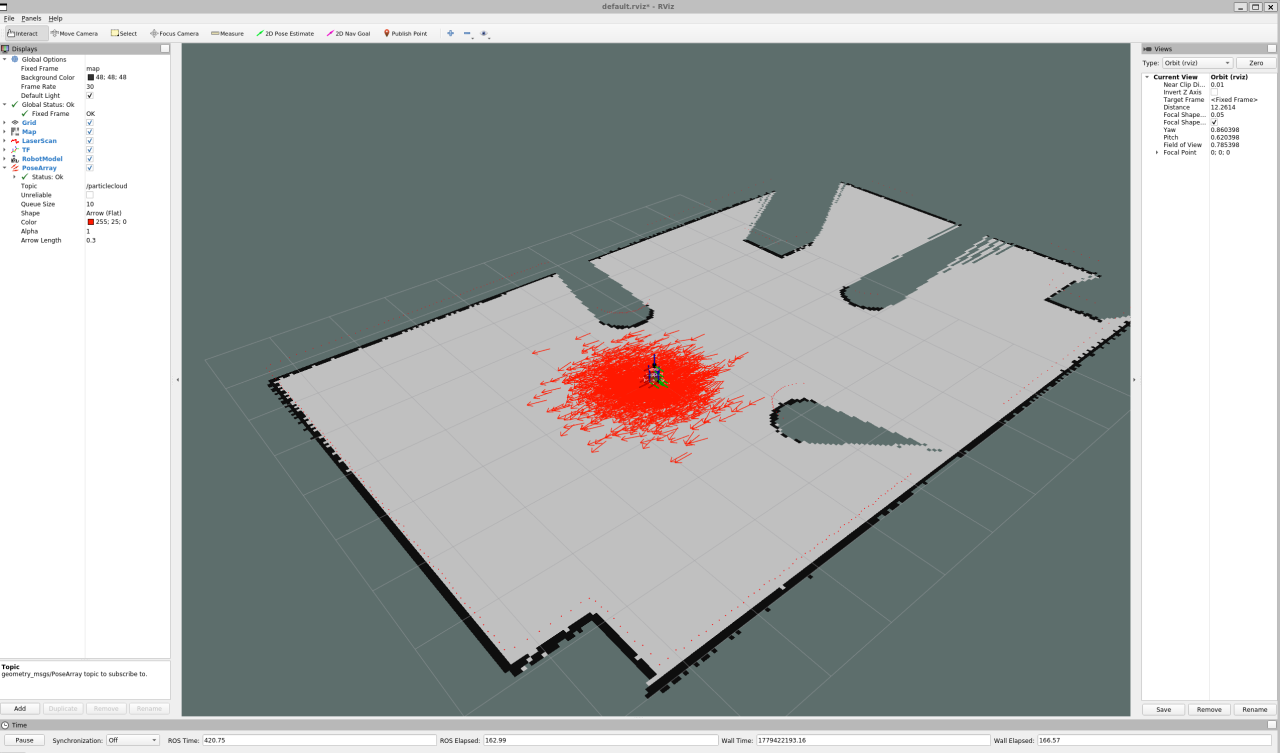
\includegraphics[width=\linewidth]{lab34_particlecloud_initial.png}
    \caption{粒子云初始分布}
  \end{subfigure}
  \hfill
  \begin{subfigure}{0.32\linewidth}
    \centering
    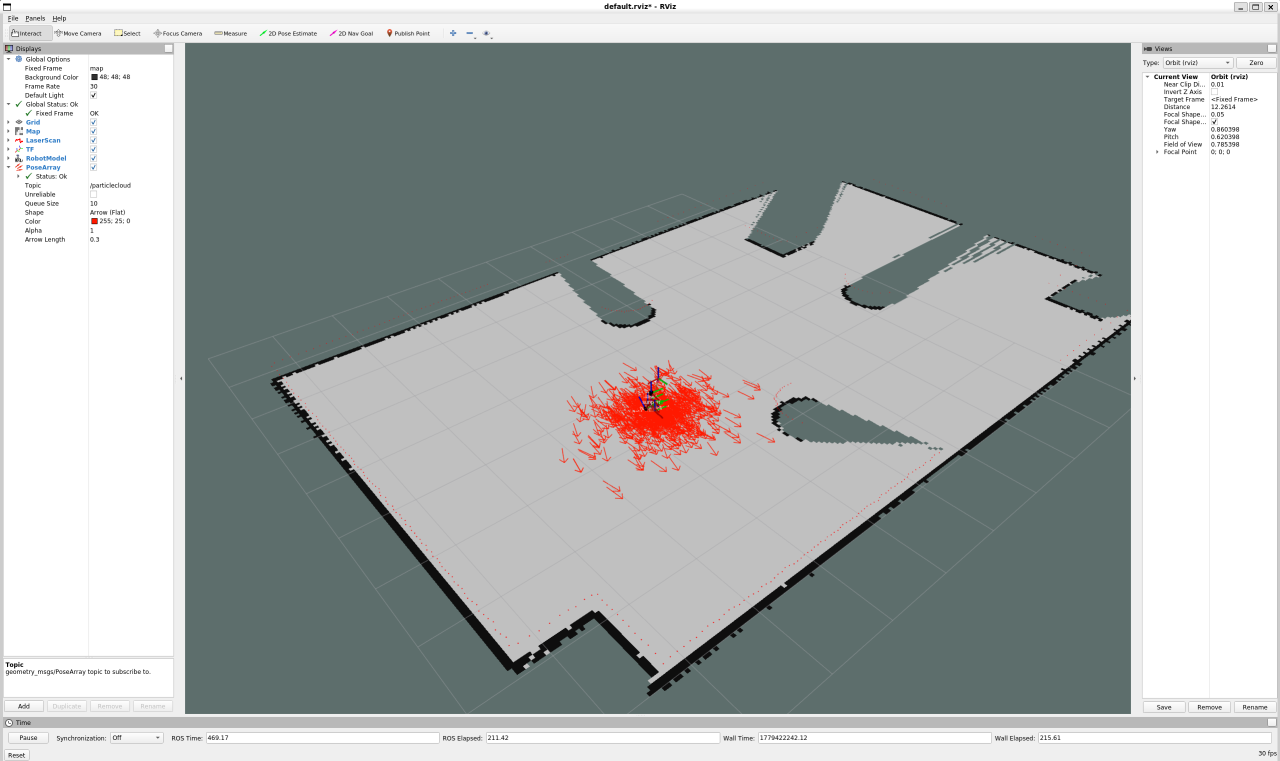
\includegraphics[width=\linewidth]{lab34_particlecloud_converged.png}
    \caption{粒子云逐步收敛}
  \end{subfigure}
  \caption{实验 4 AMCL 定位与粒子云变化。}
  \label{fig:amcl-sim}
\end{figure}

\subsection{定位跟踪与鲁棒性观察}

在实车地图上，AMCL 的粒子云会随着机器人运动而更新。若初始位姿偏差较大，可以先用 RViz 的 \verb|2D Pose Estimate| 给出近似初值；机器人继续移动后，激光扫描与地图边界不断匹配，粒子云会重新集中。图 \ref{fig:amcl-real} 展示了实车地图上的定位状态：红色粒子云聚集在机器人周围，激光点与地图边界基本一致，说明定位结果可用于后续导航。

\begin{figure}[H]
  \centering
  \begin{subfigure}{0.49\linewidth}
    \centering
    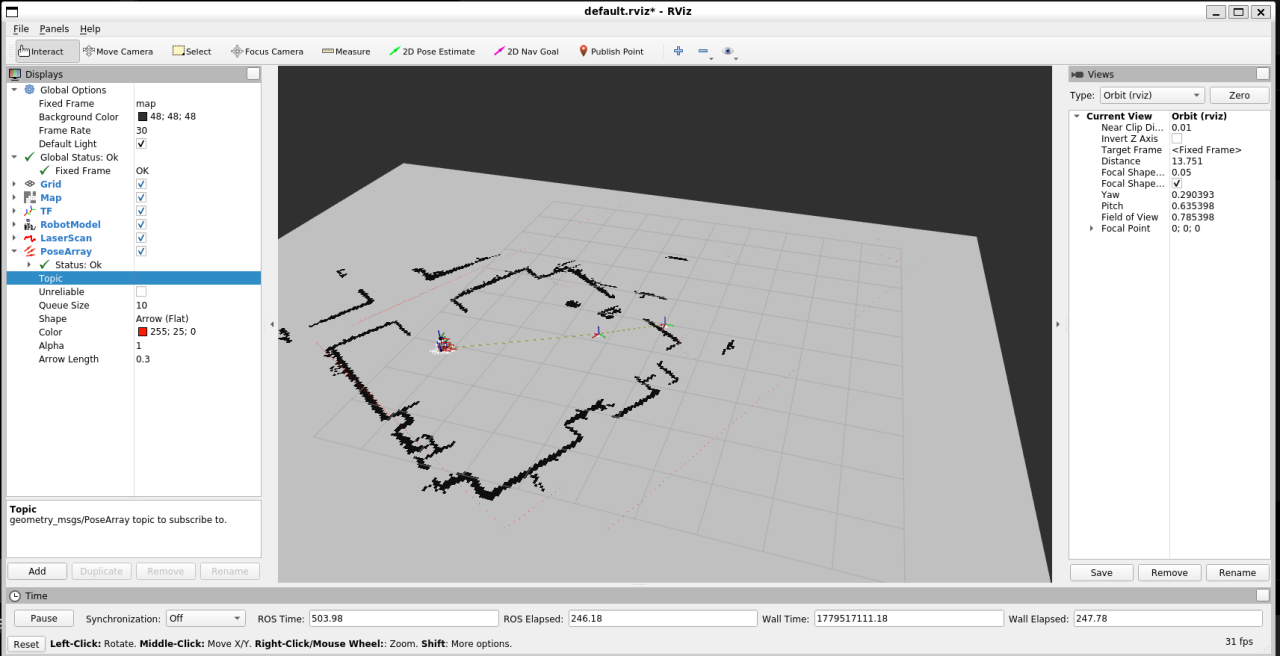
\includegraphics[width=\linewidth]{lab34_real_map_scan_start.png}
    \caption{实车地图与扫描点}
  \end{subfigure}
  \hfill
  \begin{subfigure}{0.49\linewidth}
    \centering
    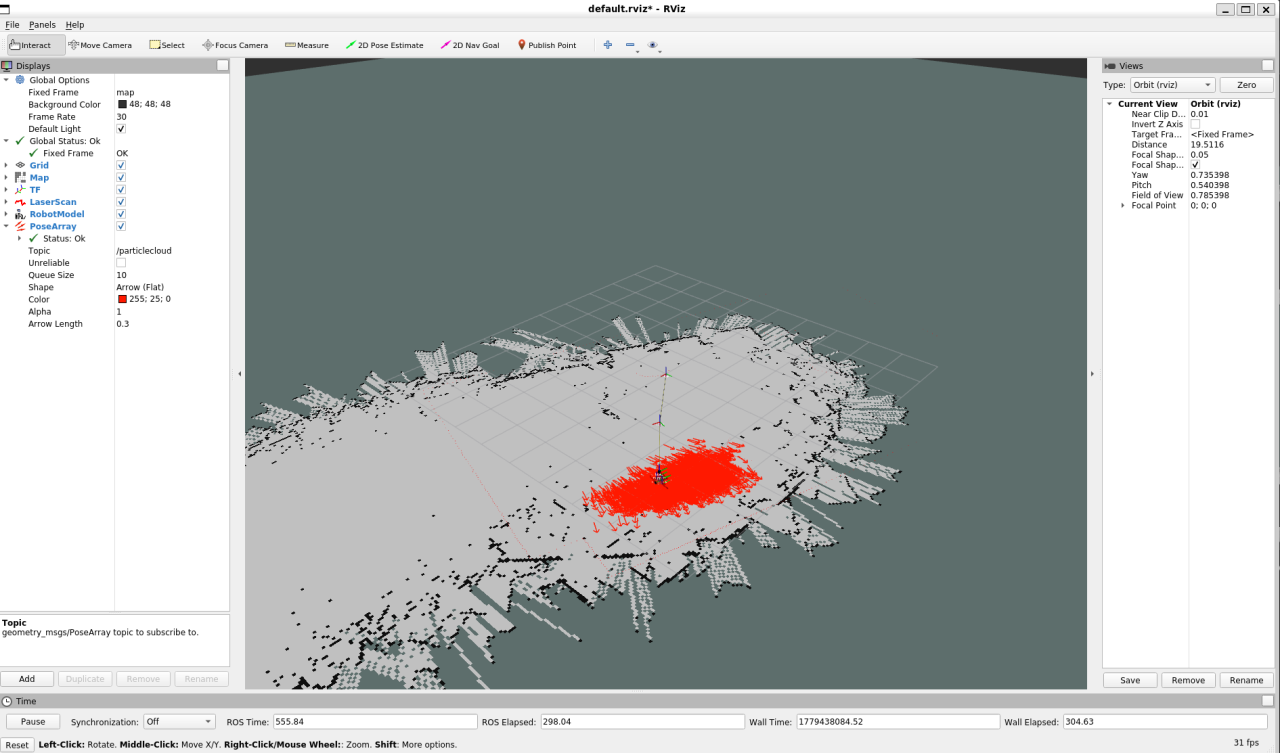
\includegraphics[width=\linewidth]{lab34_real_localization_motion_b.png}
    \caption{运动后的粒子云跟踪}
  \end{subfigure}
  \caption{实车地图中的定位跟踪结果。}
  \label{fig:amcl-real}
\end{figure}

定位效果不能只看机器人模型是否出现在地图中，还要同时检查激光扫描是否贴合障碍物边界、粒子云是否收敛、TF 树是否连通。如果 \verb|odom -> base_footprint| 缺失，AMCL 无法根据运动更新粒子；如果 \verb|map -> odom| 不稳定，机器人在全局地图中的位姿会跳变。

\section{结论与问题讨论}

实验 3 完成了仿真和实车场景下的二维地图构建，并保存了后续定位与导航使用的 \verb|nav.pgm|、\verb|nav.yaml|；实验 4 在该静态地图上完成了 AMCL 定位验证，观察到粒子云从分散到收敛，激光扫描与地图障碍物边界基本吻合。由此说明地图、雷达、里程计和 TF 链路已经能够支撑后续路径规划实验。

\textbf{URDF、RViz、Gazebo 的作用。}
URDF 描述机器人 link、joint 和传感器安装关系；Gazebo 负责物理仿真和传感器仿真；RViz 负责显示 ROS 数据，如地图、激光、TF、机器人模型和粒子云。Gazebo 更像运行实验世界，RViz 更像观察机器人系统内部状态。

\textbf{雷达静态 TF 错误的影响。}
如果 \verb|base_footprint| 到雷达坐标系的平移或旋转错误，激光点会投影到错误位置，建图阶段会产生墙体偏移、障碍物重影和地图变形；定位阶段会导致 AMCL 观测模型评分错误，粒子云难以收敛或收敛到错误位姿。

\textbf{Gmapping 与 Hector 的区别。}
\verb|gmapping| 通常结合里程计和激光数据，适合仿真或里程计较可靠的平台；\verb|hector_mapping| 更依赖激光扫描匹配，对高频雷达友好，在实车里程计噪声较大时更容易得到可用地图。两者都会围绕 \verb|map|、\verb|odom|、\verb|base_footprint| 和雷达坐标系组织数据。

\textbf{map、odom、base\_footprint 的关系。}
\verb|map| 是全局静态地图坐标系，允许定位算法进行全局修正；\verb|odom| 是局部连续坐标系，短时间平滑但长期会漂移；\verb|base_footprint| 是机器人底盘坐标系。链式结构 \verb|map -> odom -> base_footprint| 把全局修正和局部连续运动分开，避免 AMCL 直接修正底盘位姿造成控制跳变。

\textbf{不同算法负责的 TF 段。}
轮式里程计或 RF2O 通常发布 \verb|odom -> base_footprint|；AMCL 根据静态地图和激光扫描发布 \verb|map -> odom|；SLAM 算法在建图时估计机器人与地图之间的关系。若使用 RF2O 配合 Gmapping 实车建图，需要先保证雷达、底盘和静态 TF 正确，再让 Gmapping 使用 RF2O 提供的里程计链。

\end{document}
